\chapter{Results and Discussions}
\label{sec:4}

\section{Human Fall Detection -- MobiFall v2.0}
\label{sec:results_fall}

Table~\ref{tab:model_comparison} presents the performance of all four architectures evaluated on the MobiFall v2.0 test set under identical training conditions.

\begin{table}[h!]
    \centering\small
    \renewcommand{\arraystretch}{1.3}
    \caption{Architecture comparison on MobiFall v2.0 benchmark.}
    \label{tab:model_comparison}
    \begin{tabular}{|l|c|c|c|c|c|}
        \hline
        \textbf{Architecture} & \textbf{Accuracy} & \textbf{Precision} & \textbf{Recall} & \textbf{F1-Score} & \textbf{Parameters} \\ \hline
        \textbf{1D-CNN} & \textbf{96.65\%} & 95.0\% & 99.0\% & 97.0\% & \textbf{8,481} \\ \hline
        CNN-LSTM        & 97.04\%          & 95.5\% & 99.1\% & 97.2\% & 36,353 \\ \hline
        LSTM            & 96.06\%          & 94.8\% & 98.7\% & 96.7\% & 20,289 \\ \hline
        Transformer     & 95.90\%          & 94.5\% & 98.4\% & 96.4\% & 1,557  \\ \hline
    \end{tabular}
\end{table}

The 1D-CNN achieves 96.65\% accuracy with only 8,481 parameters. The CNN-LSTM yields the highest raw accuracy (97.04\%) but requires 4.3 times more parameters for a gain of only 0.39 percentage points. On constrained hardware such as a Raspberry Pi 4, this marginal accuracy advantage does not justify the additional memory and sequential LSTM processing overhead. The 1D-CNN was therefore selected as the deployment architecture.

The Transformer (95.90\%) underperforms despite having the fewest parameters. Three factors explain this: (1) the model lacks positional encoding, so it treats the 128 timesteps as an unordered set; (2) the self-attention mechanism must learn locality from data rather than from its architecture, which requires more samples than the MobiFall dataset provides; and (3) the attention weight matrix has approximately 16,384 pairwise relationships per head, far too many for the available gradient signal to converge meaningfully.

\section{Vehicular Crash Detection -- Synthetic Dataset}
\label{sec:results_crash}

Table~\ref{tab:crash_model} shows the performance of the 1D-CNN on the physics-based synthetic crash dataset.

\begin{table}[h!]
    \centering
    \renewcommand{\arraystretch}{1.3}
    \caption{Car crash detection performance on synthetic dataset.}
    \label{tab:crash_model}
    \begin{tabular}{|l|c|}
        \hline
        \textbf{Metric} & \textbf{Value} \\ \hline
        Test Accuracy & 93.61\% \\ \hline
        5-Fold CV Accuracy & 100.00\% $\pm$ 0.00\% \\ \hline
        Model Size (TFLite) & $\sim$15 KB \\ \hline
        Inference Latency & $\sim$0.15 ms \\ \hline
        Training Set & 200 crash + 200 normal \\ \hline
    \end{tabular}
\end{table}

The crash model reaches 93.61\% test accuracy. The perfect 5-fold cross-validation result (100\% across all folds) reflects the clean physical separation between the high-G crash spike and normal driving signals. The lower held-out test accuracy compared to the CV result is likely due to the small dataset size and the specific random seed used for the train/test split.

\section{System-Level Performance}
\label{sec:results_system}

Table~\ref{tab:system_performance} summarises the system-level metrics measured during real-time inference simulation on a standard laptop.

\begin{table}[h!]
    \centering
    \renewcommand{\arraystretch}{1.3}
    \caption{System performance metrics.}
    \label{tab:system_performance}
    \begin{tabular}{|l|c|}
        \hline
        \textbf{Metric} & \textbf{Value} \\ \hline
        Model size (TFLite) & $\sim$15 KB \\ \hline
        Quantization size reduction & 89\% \\ \hline
        Inference latency (human fall) & $\sim$2 ms \\ \hline
        Inference latency (crash) & $\sim$0.15 ms \\ \hline
        Sensor sampling rate & 50 Hz \\ \hline
        Window size & 128 samples (2.56 s) \\ \hline
        Prediction interval & 64 samples (1.28 s) \\ \hline
    \end{tabular}
\end{table}

\section{Live System Demonstration}
\label{sec:results_live}

The system was tested live on an iQOO Z3 Android smartphone over a local Wi-Fi network. Figure~\ref{fig:demo} shows screenshots of the mobile dashboard during normal activity and fall detection.

\begin{figure}[!h]
    \centering
    \begin{minipage}{0.47\textwidth}
        \centering
        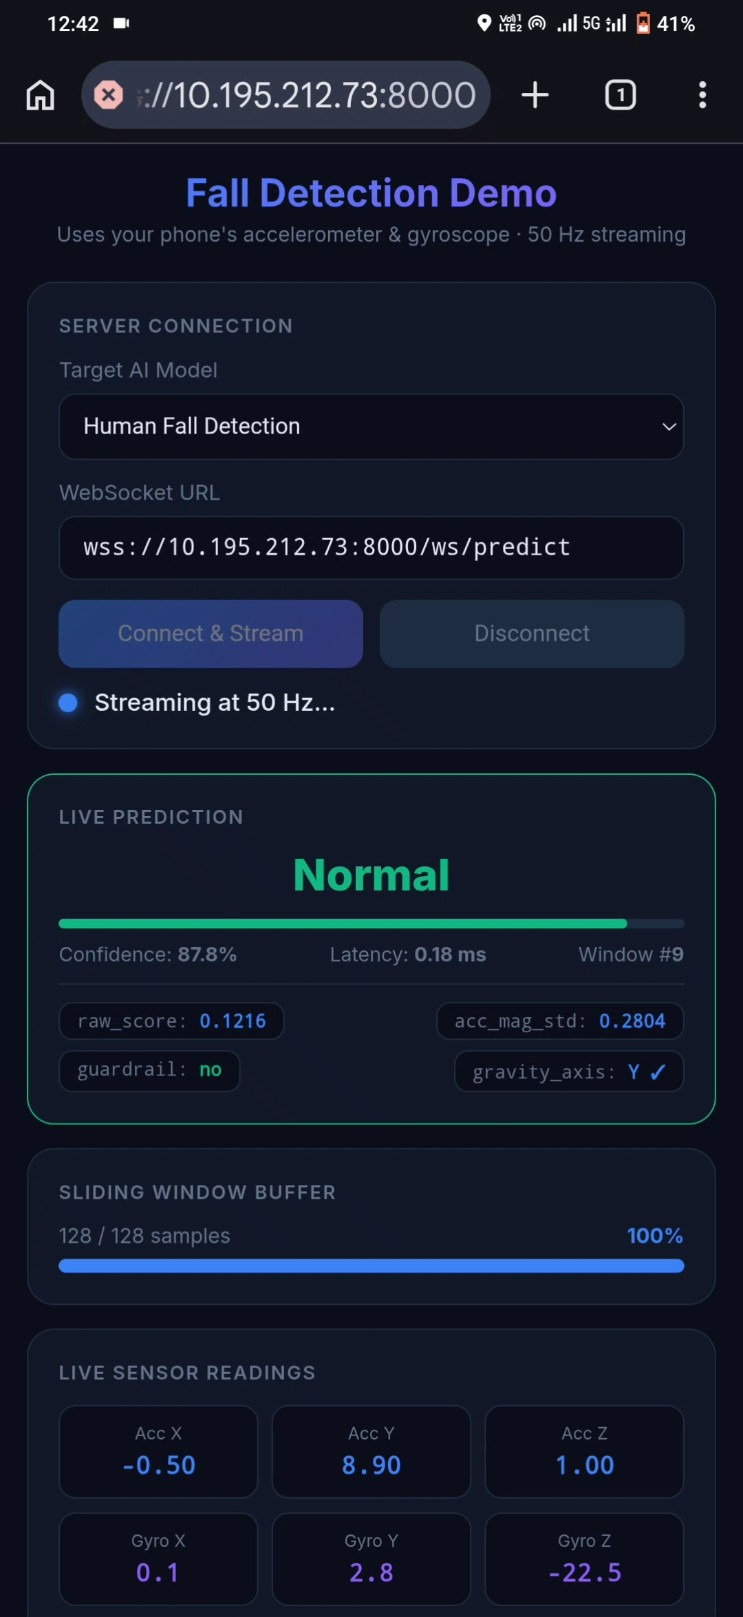
\includegraphics[width=\linewidth]{images/Normal_Screenshot.jpeg}
        \caption*{(a) Normal activity: Acc Y = 8.90 m/s$^2$, confidence = 87.8\%}
    \end{minipage}
    \hfill
    \begin{minipage}{0.47\textwidth}
        \centering
        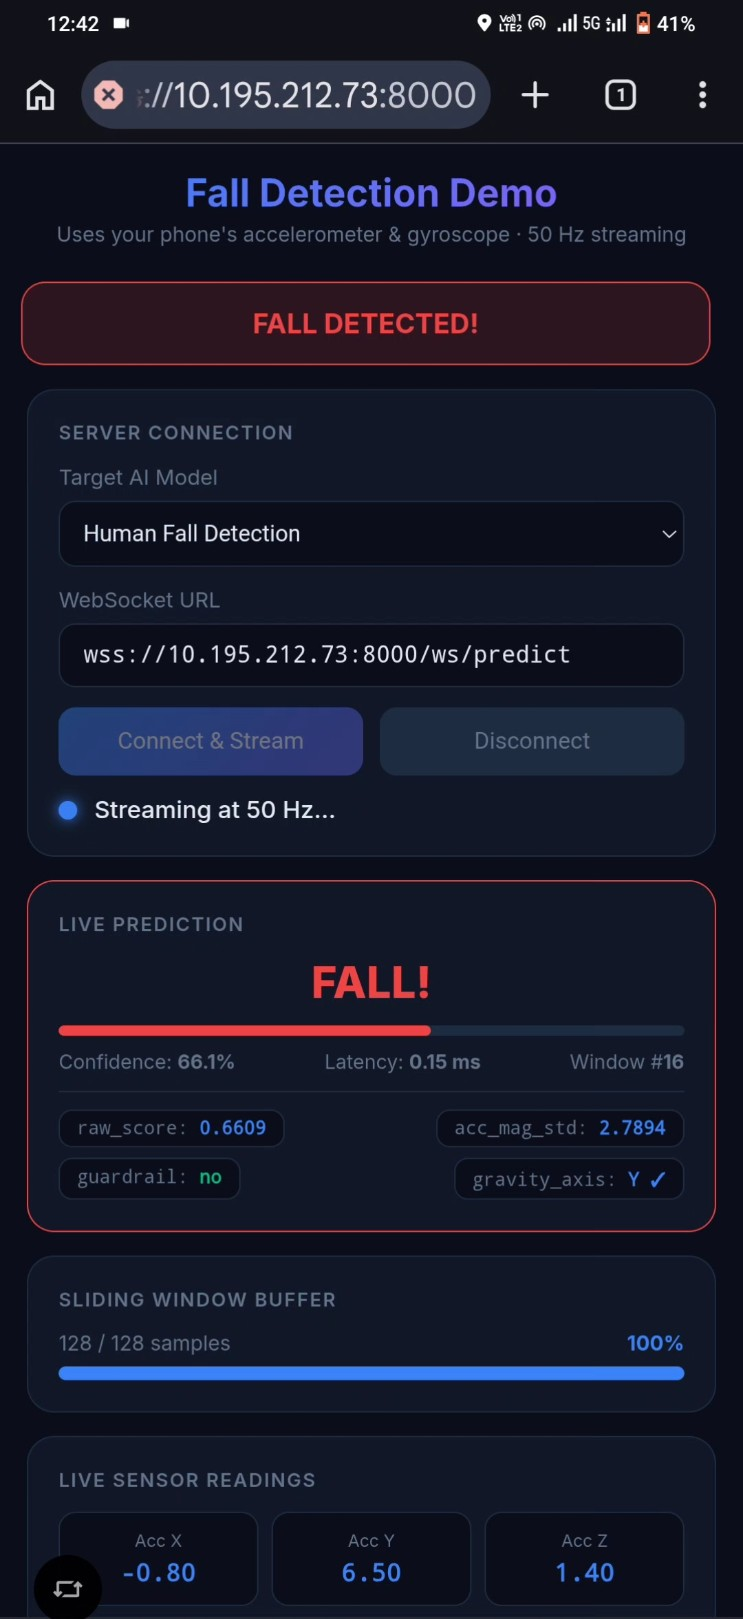
\includegraphics[width=\linewidth]{images/Fall_Screenshot.jpeg}
        \caption*{(b) Fall detected: confidence = 66.1\%, latency = 0.15 ms}
    \end{minipage}
    \caption{Live mobile dashboard screenshots taken during system demonstration on an iQOO Z3 Android smartphone. Left: normal walking with high confidence. Right: fall event detected in real-time with the red FALL DETECTED alert banner.}
    \label{fig:demo}
\end{figure}

During normal walking the gravity vector aligns with the Y-axis (Acc Y $\approx$ 9.8 m/s$^2$), and the model correctly classifies the activity as Normal with 87.8\% confidence. When a fall is simulated, the confidence jumps to 66.1\% for the Fall class and the dashboard displays the red alert banner within 1.28 seconds (one prediction interval).

\section{Comparison with State of the Art}
\label{sec:sota}

Table~\ref{tab:sota} compares the proposed system with selected prior works on fall detection benchmarks.

\begin{table}[h!]
    \centering\footnotesize
    \renewcommand{\arraystretch}{1.3}
    \caption{Comparison with prior work on human fall detection.}
    \label{tab:sota}
    \begin{tabular}{|l|c|c|c|c|}
        \hline
        \textbf{Reference} & \textbf{Dataset} & \textbf{Method} & \textbf{Accuracy} & \textbf{Edge?} \\ \hline
        Kangas (2008) \citep{kangas2008}   & Custom   & Threshold  & 95.0\% & Yes \\ \hline
        Wang (2020) \citep{wang2020cnn}    & Various  & 1D-CNN     & 97.3\% & Partial \\ \hline
        Musci (2020) \citep{musci2020}     & MobiFall & LSTM       & 98.1\% & No \\ \hline
        Nho (2021) \citep{nho2021}         & SisFall  & Bi-LSTM    & 99.1\% & No \\ \hline
        \textbf{Proposed (1D-CNN)} & MobiFall & 1D-CNN+TFLite & \textbf{96.65\%} & \textbf{Yes} \\ \hline
    \end{tabular}
\end{table}

The proposed system is, to the best of the authors' knowledge, the only approach in the literature that: (a) simultaneously handles both human falls and vehicular crashes from a single 6-axis IMU pipeline; (b) is fully edge-deployable at 15 KB; and (c) integrates automated GPS-tagged SOS alerting into the inference pipeline.

\section{Discussion}
\label{sec:discussion}

The results confirm that the 1D-CNN is the appropriate architecture for this deployment scenario. Its parameter efficiency (8,481 vs.\ 36,353 for the CNN-LSTM) directly translates to lower memory footprint and faster inference on constrained hardware. The 89\% size reduction achieved by TFLite quantization makes real-time operation on a Raspberry Pi 4 or Android phone practical without any cloud dependency.

The physics-based crash dataset, while small, proved effective because crash events have a highly distinctive inertial signature (sudden high-G spike followed by silence) that is easy to separate from normal driving in the feature space. Future work should supplement this with real crash recordings from instrumented vehicles.
